\documentclass{article}
\usepackage{amsmath} % Required for typesetting matrices
\usepackage{amssymb} % Required for using the "therefore" symbol
\usepackage{graphicx}

\title{Matrix, Linear Algebra, Differential Equation \\ MAT 2207}
\author{Jannat Tohfa Chowdhury}
\date{April 2024}

\begin{document}
\maketitle
\newpage
% Your lectures start here
\section*{Matrix}
\subsection*{Definition of Matrix: }
\vspace{10pt}
A system of any \( m \times n \) numbers arranged in a rectangular arrangement of \( m \) rows and \( n \) columns is called a matrix of order \( m \times n \) or an \( m \times n \) matrix.
    \paragraph{Ex:}
    \[
    \begin{minipage}{0.6\textwidth}
    \[
    \begin{bmatrix}
    1 & -2 & 4 \\
    3 & 1 & 7 \\
    \end{bmatrix}
    \]
    \end{minipage}
    \begin{minipage}{0.4\textwidth}
    is a $2 \times 3$ matrix.
    \end{minipage}
    \]
    \vspace{12pt}
    \textbf{in general form:}
    \[
    A = 
    \begin{bmatrix}
    \sigma_{11} & \sigma_{12} & \cdots & \sigma_{1n} \\
    \sigma_{21} & \sigma_{22} & \cdots & \sigma_{2n} \\
    \vdots & \vdots & \vdots & \vdots \\
    \sigma_{m1} & \sigma_{m2} & \cdots & \sigma_{mm}
    \end{bmatrix}
    =(\sigma_{ij})_{mxm}
    \]
\vspace{20pt}
\subsection*{Singular and Non-singular Matrix:}
\vspace{10pt}
    Let \( A \) be any square matrix. If \( \det(A) = 0 \), then \( A \) is called a singular matrix, and if \( \det(A) \neq 0 \), then \( A \) is called a non-singular matrix.
    \vspace{12pt}
    \paragraph{Ex:}
    \begin{minipage}{0.4\textwidth}
    \[ A = 
    \begin{bmatrix}
    1 & 2 \\
    2 & 4 \\
    \end{bmatrix} \]
    \end{minipage}
    \begin{minipage}{0.1\textwidth}
    \end{minipage} 
    \begin{minipage}{0.4\textwidth}
    \[ B = 
    \begin{bmatrix}
    1 & 5 \\
    2 & 12 \\
    \end{bmatrix} \]
    \end{minipage}

    \vspace{20pt}    
    Then \(|A| = \det(A) = \det \begin{bmatrix} 1 & 2 \\ 2 & 4 \end{bmatrix} = 4 - 4 = 0\)
    
    So, \(A\) is a singular matrix
    
    \vspace{20pt}
    Again, \(|B| = \det(B) = \det \begin{bmatrix} 1 & 5 \\ 2 & 12 \end{bmatrix} = 12 - 10 = 2 \neq 0\)
    
    Hence, \( B \) is a non-singular matrix.
\vspace{20pt}
\subsection*{Inverse Matrix:}
\vspace{10pt}
    Let \( A \) and \( B \) be two \(n \times n\) square matrices such that \( AB = BA = I_{n} = I \), then \( B \) is said to be the inverse of \( A \), and we write \( B = A^{-1} \). Also, \( A = B^{-1} \).
    \vspace{20pt}
    \paragraph{Ex:}
    Let \( A = \begin{bmatrix} 4 & 3 \\ 1 & 1 \end{bmatrix} \) and \( B = \begin{bmatrix} 1 & -3 \\ -1 & 4 \end{bmatrix} \).
    
    \vspace{10pt}
    
    \begin{minipage}{.45\textwidth}
    \(\therefore\ AB = 
    \begin{bmatrix} 4 & 3 \\ 1 & 1 \end{bmatrix}
    \times
    \begin{bmatrix} 1 & -3 \\ -1 & 4 \end{bmatrix}\)
    \end{minipage}

    
    \vspace{10pt}
    
    \begin{minipage}{0.7\textwidth}
    \[ = \begin{bmatrix} 4 - 3 & -12 + 12 \\ 1 - 1 & -3 + 4 \end{bmatrix} = \begin{bmatrix} 1 & 0 \\ 0 & 1 \end{bmatrix} = I_{2} \]
    \end{minipage}
    
    \vspace{10pt}
    
    \begin{minipage}{0.6\textwidth}
    and \( BA = \begin{bmatrix} 1 & -3 \\ -1 & 4 \end{bmatrix} \times \begin{bmatrix} 4 & 3 \\ 1 & 1 \end{bmatrix} \)
    \end{minipage}
    
    \vspace{10pt}

    \begin{minipage}{0.7\textwidth}
        \[ = \begin{bmatrix} 4 - 3 & 3 - 3 \\ -4 + 4 & -3 + 4 \end{bmatrix} = \begin{bmatrix} 1 & 0 \\ 0 & 1 \end{bmatrix} = I_{2} \]
    \end{minipage}
   
    \vspace{10pt}
    
    \(\therefore\)\(AB = BA = I_{2} = I\)
    
    Therefore, we can write \( A = B^{-1} \) and \( B = A^{-1} \).

    \vspace{30pt}
    [N.B.: The inverse of a matrix exists only when the matrix is non-singular,

i.e., \( |A| \neq \emptyset \).]

    *** Multiplication of two matrices is possible only when the number of columns in the first matrix is equal to the number of rows in the second matrix.

\vspace{20pt}

\subsection*{Echelon Matrix:}
    \vspace{10pt}
    Let \( A = (a_{ij})_{m \times n} \) be any matrix. Then \( A \) is said to be an echelon matrix or is said to be in echelon form if:
    \begin{enumerate}
        \item all the non-zero rows (if any) precede the zero rows,
        \item the number of zero entries preceding the first non-zero entry in each row increases by row.
    \end{enumerate}

    \vspace{10pt}

    \paragraph{Ex:}
    \[\begin{bmatrix} 1 & -1 & 2 \\ 0 & 3 & 2 \\ 0 & 0 & 5 \end{bmatrix} \text{ is an echelon matrix,  but } \begin{bmatrix} 1 & 2 & 3 \\ 0 & -1 & 3 \\ 2 & 5 & 4 \end{bmatrix} \text{ is not an echelon matrix.}\]

    \vspace{20px}

\subsection*{Rank of a Matrix:}
    \vspace{10pt}
    Rank of a matrix is the largest non-zero row in the matrix of row echelon form.

    \paragraph{Ex:}
    \begin{minipage}{0.45\textwidth}
    \[ A = \begin{bmatrix} 1 & 4 & 5 \\ 0 & 3 & 7 \\ 0 & 0 & 6 \end{bmatrix} \]
    \end{minipage}
    \begin{minipage}{0.45\textwidth}
        \[ B = \begin{bmatrix} 1 & 2 & 3 \\ 0 & 6 & 7 \\ 0 & 0 & 0 \end{bmatrix} \]
    \end{minipage}

    \vspace{20pt}
    \text{Rank of matrix } A = 3, \quad \text{Rank of matrix } B = 2

    \vspace{60pt}
    \textbf{Find the rank of the following matrices:}
    
    \begin{center}
    \begin{minipage}{0.45\textwidth}
    \[ A = \begin{bmatrix} 1 & -1 & -1 & 2 \\ 2 & 1 & 3 & -1 \\ 3 & 2 & 1 & 2 \\ 4 & 1 & 2 & 3 \end{bmatrix} \]
    \end{minipage}
    \hspace{0.05\textwidth}
    \begin{minipage}{0.45\textwidth}
    \[ B = \begin{bmatrix} 1 & 3 & 1 & -2 & -3 \\ 1 & 4 & 3 & -1 & -4 \\ 2 & 3 & -4 & -7 & -3 \\ 3 & 8 & 1 & -7 & -8 \end{bmatrix} \]
    \end{minipage}
    \end{center}
    
    \vspace{1em}
    
    \begin{center}
    \begin{minipage}{0.45\textwidth}
    \[ C = \begin{bmatrix} 1 & -1 & 2 & 1 \\ 3 & 0 & 2 & 2 \\ 2 & 1 & -1 & 1 \\ 1 & 0 & 1 & 1 \end{bmatrix} \]
    \end{minipage}
    \hspace{0.05\textwidth}
    \begin{minipage}{0.45\textwidth}
    \[ D = \begin{bmatrix} 1 & -1 & 1 & 3 \\ 2 & -1 & 0 & 2 \\ 1 & 0 & 1 & 1 \\ 4 & 2 & 0 & 1 \end{bmatrix} \]
    \end{minipage}
    \end{center}

    \vspace{120pt}

    \begin{figure}[htbp]
        \centering
        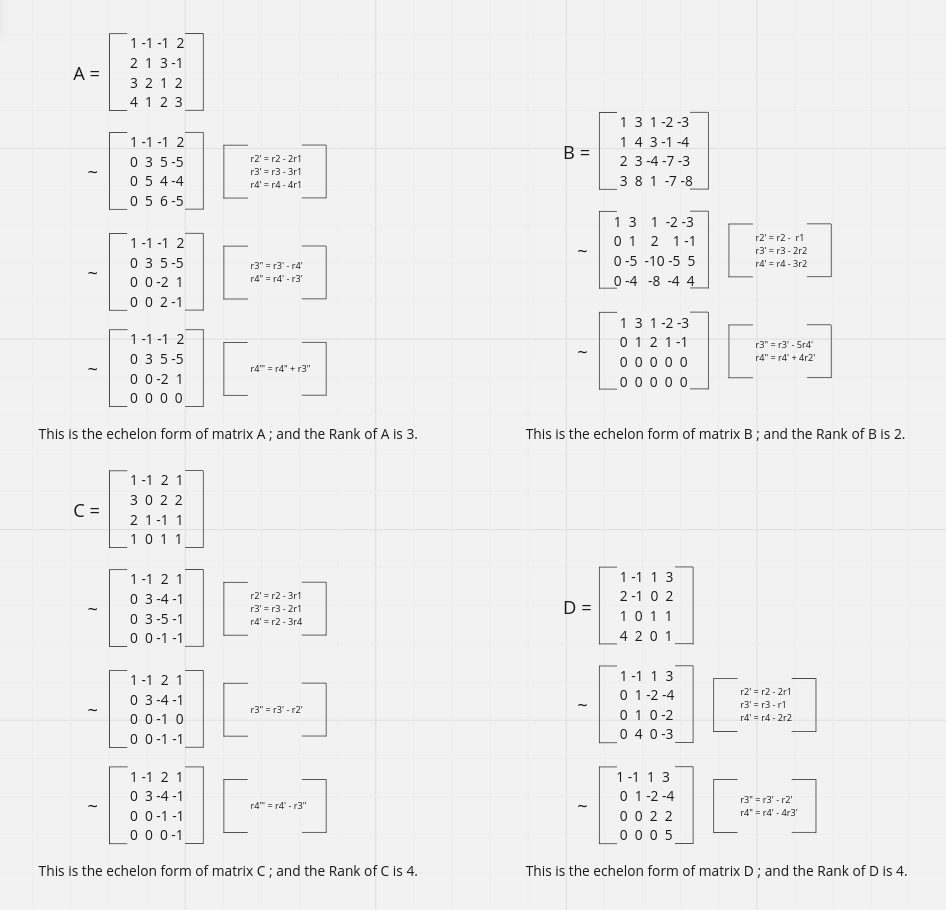
\includegraphics[width=1.2\textwidth, height=.95\textheight]{../Asset/rankOfExc.png}
        \label{fig:example}
    \end{figure}
    
    \newpage
    \section*{Inverse Matrix Calculation:}
    \vspace{10pt}
    Find the inverse of the matrix by using the formula [A:I]

    \vspace{10pt}
    example; find the inverse matrix of \( A = \begin{bmatrix} 1 & -1 & 2 & 1 \\ 3 & 0 & 2 & 2 \\ 2 & 1 & -1 & 1 \\ 1 & 0 & 1 & 1 \end{bmatrix} \)

    \vspace{10pt}
    Solution:
    \vspace{10pt}
    \begin{figure}[htbp]
        \centering
        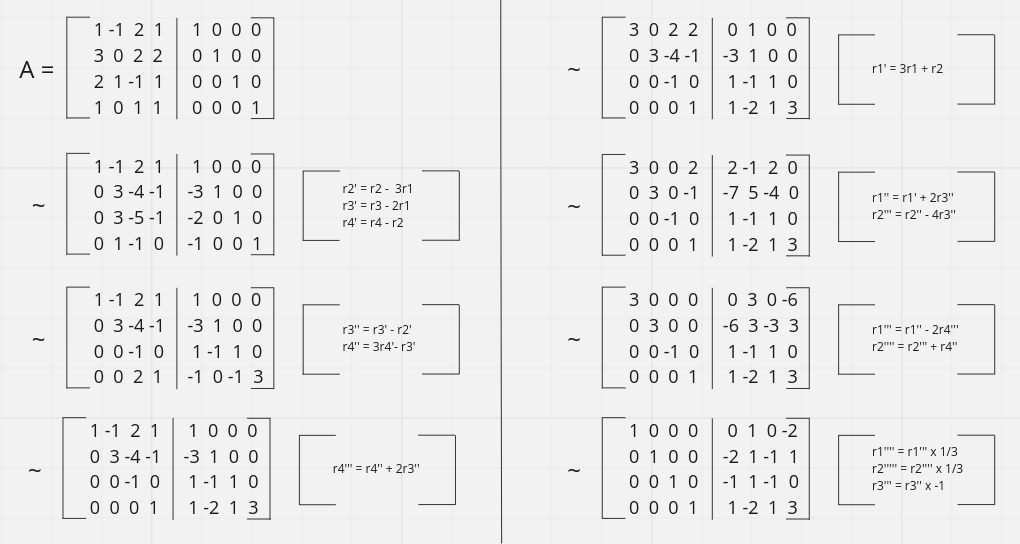
\includegraphics[width=1.2\textwidth, height=.7\textheight]{../Asset/invEXA.png}        \label{fig:example}
    \end{figure}

    \vspace{10pt}
    \newpage
    \underbar{Home Work:}

    find the inverse matrix of
    \hspace*{10pt}
    \( B = \begin{bmatrix} -1 & 2 & -3 \\ 2 & 1 & 0 \\ 4 & -2 & 5 \end{bmatrix} \);  
    \( C = \begin{bmatrix} 1 & 3 & 1 & 1 \\ 2 & 5 & 2 & 2 \\ 1 & 3 & 8 & 9 \\ 1 & 3 & 2 & 2 \end{bmatrix} \)
    
    \begin{figure}[htbp]
        \centering
        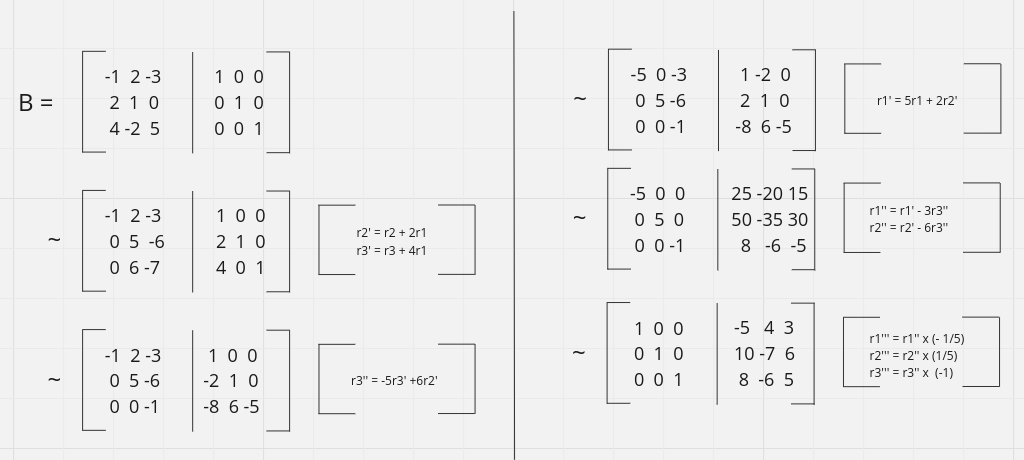
\includegraphics[width=1.2\textwidth, height=.7\textheight]{../Asset/invHWB.png}
        \label{fig:example}
    \end{figure}
    \begin{figure}[htbp]
        \centering
        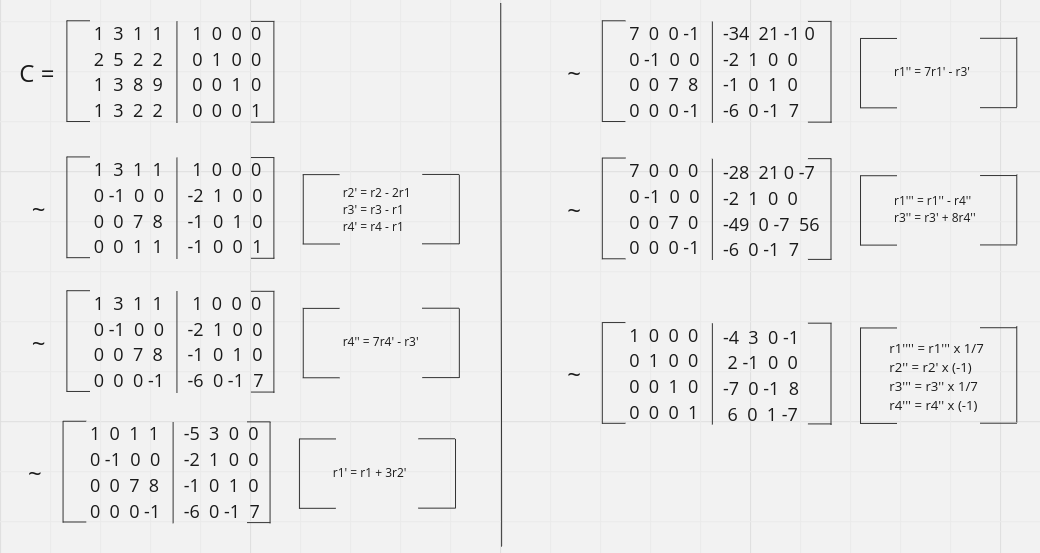
\includegraphics[width=1.2\textwidth, height=.7\textheight]{../Asset/invHWC.png}
        \label{fig:example}
    \end{figure}

    \newpage
    \section*{Eigenvalues and Eigenvectors:}
    
    \vspace{10pt}
    A nonzero matrix \( X \) is an eigenvector of a square matrix \( A \) if there exists a \( \lambda \) such that \( AX = \lambda X \). Then \( X \) is called the eigenvector of \( A \) with eigenvalue \( \lambda \) and \( \lambda \) is called the eigenvalue of \( A \).
    
    \vspace{10pt}
    The equation \( |A - \lambda I| = 0\) is called the characteristic equation of \( A \).
    
    \vspace{10pt}
    Cayley-Hamilton theorem states that every square matrix A satisfies it's characteristic equation.

    \vspace{10pt}
    \subsection*{Example:}
        Find the eigenvalues and eigenvectors of the matrix \( A = \begin{bmatrix} 1 & 4 \\  2 & 3  \end{bmatrix} \) in the field of real numbers ( \( \mathbb{R} \) ). Also verify the Cayley-Hamilton theorem.

    \vspace{20pt}
    \textbf{\underline{\textit{Sol}}$_{\textit{n}}$}:

    \vspace{10pt}
    Given matrix, \(A = \begin{bmatrix} 1 & 4 \\  2 & 3  \end{bmatrix}\)
    
    \vspace{10pt}
    Characteristic matrix of A inverse:

    \[
    \begin{aligned}
        A - \lambda I &= 
        \begin{bmatrix}
            1 & 4 \\
            2 & 3
        \end{bmatrix}
        - \lambda
        \begin{bmatrix}
            1 & 0 \\
            0 & 1
        \end{bmatrix} \\
        &= \begin{bmatrix}
                1-\lambda & 4 \\
                2 & 3-\lambda
            \end{bmatrix}
    \end{aligned}
    \]
    \vspace{20pt}

    Characteristic equation of A inverse:

    \vspace{10pt}
    \(|A - \lambda I| = 0 \)

    or,
    \[
    \left|
    \begin{array}{cc}
        1 - \lambda & 4 \\
        2 & 3 - \lambda
    \end{array}
    \right| = 0
    \]

    or,
    \((1 - \lambda)(3 - \lambda) - 8 = 0 \)

    or,
    \(3 - 4\lambda + \lambda^2 - 8 = 0 \)

    or,
    \( \lambda^2 - 4\lambda - 5 = 0 \)

    or,
    \( \lambda^2 - 5\lambda + \lambda - 5 = 0 \)

    or
    \( \lambda = 1 \) or \( \lambda = -5 \)

    \vspace{10pt}
    thus, \( \lambda = 1, -5 \); 

    these are the eigenvalues of \( A \).

    \newpage

    For \(x = 5\), 

    \[
    \begin{aligned}
        (A - \lambda I) v &= 0 \\
        \text{or,} \quad &\begin{bmatrix}
            1-5 & 4 \\
            2 & 3-5
        \end{bmatrix} \begin{bmatrix}
            x_1 \\
            x_2
        \end{bmatrix} = 0 \\
        \text{or,} \quad &\begin{bmatrix}
            -4 & 4 \\
            2 & -2
        \end{bmatrix} \begin{bmatrix}
            x_1 \\
            x_2
        \end{bmatrix} = 0
    \end{aligned}
    \]
    
    Now, we can write,
    
    \[
    \begin{aligned}
        -4x_1 + 4x_2 &= 0 \\
        2x_1 - 2x_2 &= 0 \\
        \text{or,} \quad &\begin{bmatrix}
            -4 & 4 \\
            2 & -2
        \end{bmatrix} \begin{bmatrix}
            x_1 \\
            x_2
        \end{bmatrix} = \begin{bmatrix}
            0 \\
            0
        \end{bmatrix} \\
        \sim \quad &\begin{bmatrix}
            -4 & 4 \\
            0 & 0
        \end{bmatrix} \quad [r_2' = 2r_2 + r_1] \\
        \sim \quad &\begin{bmatrix}
            -1 & 1 \\
            0 & 0
        \end{bmatrix} \quad [r_1' = r_1 \times \frac{1}{4}]
    \end{aligned}
    \]
    
    \vspace{10pt}
    From this first row,
    
    \[
    \begin{aligned}
        -x_1 + x_2 &= 0 \\
        x_1 &= x_2 = s \quad (\text{say})
    \end{aligned}
    \]
    
    Taking \(s = 1\), the eigenvector can be written as,
    
    \[
    v_1 = \begin{bmatrix}
        1 \\
        1
    \end{bmatrix}
    \]
    
    Now for \(\lambda = -1\),
    
    \[
    \begin{aligned}
        (A - \lambda I) v &= 0 \\
        \text{or,} \quad &\begin{bmatrix}
            1-(-1) & 4 \\
            2 & 3-(-1)
        \end{bmatrix} \begin{bmatrix}
            x_1 \\
            x_2
        \end{bmatrix} = 0 \\
        \text{or,} \quad &\begin{bmatrix}
            2 & 4 \\
            2 & 4
        \end{bmatrix} \begin{bmatrix}
            x_1 \\
            x_2
        \end{bmatrix} = 0
    \end{aligned}
    \]
    
    \newpage
    Now, we can write,
    
    \[
    \begin{aligned}
        &2x_1 + 4x_2 = 0 \\
        &2x_1 + 4x_2 = 0 \\
        \text{or,} \quad &\begin{bmatrix}
            2 & 4 \\
            2 & 4
        \end{bmatrix} \begin{bmatrix}
            x_1 \\
            x_2
        \end{bmatrix} = \begin{bmatrix}
            0 \\
            0
        \end{bmatrix} \\
        \sim \quad &\begin{bmatrix}
            2 & 4 \\
            0 & 0
        \end{bmatrix} \quad [r_2' = r_2 - r_1] \\
        \sim \quad &\begin{bmatrix}
            1 & 2 \\
            0 & 0
        \end{bmatrix} \quad [r_1' = r_1 \times \frac{1}{2}]
    \end{aligned}
    \]
    
    \vspace{10pt}
    From this first row,
    
    \[
    \begin{aligned}
        & x_1 + 2x_2 = 0 \\
        & x_1 = -2x_2
    \end{aligned}
    \]
    
    Taking \(x_2 = 1\), we get \(x_1 = -2\). Thus, the eigenvector can be written as,
    
    \[
    v_2 = \begin{bmatrix}
        -2 \\
        1
    \end{bmatrix}
    \]
    
    \subsection*{Cayley-Hamilton proof:}
    We have to show that \( A^2 - 4A - 5I = 0 \).


    This will square the matrix \( A \), which is:

    \[ A^2 = \begin{bmatrix}
        1 & 4 \\
        2 & 3
    \end{bmatrix} \times \begin{bmatrix}
        1 & 4 \\
        2 & 3
    \end{bmatrix} = \begin{bmatrix}
        9 & 16 \\
        8 & 17
    \end{bmatrix} \]

    Now, \( A^2 - 4A - 5I = \begin{bmatrix}
        9 & 16 \\
        8 & 17
    \end{bmatrix} - \begin{bmatrix}
        4 & 16 \\
        8 & 12
    \end{bmatrix} - \begin{bmatrix}
        5 & 0 \\
        0 & 5
    \end{bmatrix}
    = \begin{bmatrix}
        0 & 0 \\
        0 & 0
    \end{bmatrix} \)
    = 0
    [Proved]

\newpage

$\delta$ Find the eigenvalues and eigenvectors of the matrix \( A = \begin{bmatrix}
    1 & -3 & 3 \\
    3 & -5 & 3  \\
    6 & -6 & 4
\end{bmatrix} \)

We know \(|A - \lambda I| = 0\)


\[or, 
\begin{array}{ccc}
\left| \begin{matrix}
1 & -3 & 3 \\
3 & -5 & 3 \\
6 & -6 & 4
\end{matrix} \right. & - & \left. \begin{matrix}
\lambda & 0 & 0 \\
0 & \lambda & 0 \\
0 & 0 & \lambda
\end{matrix} \right| = 0
\end{array}
\]

\[or, 
\begin{array}{ccc}
\left| \begin{matrix}
1-\lambda & -3 & 3 \\
3 & -5-\lambda & 3 \\
6 & -6 & 4-\lambda
\end{matrix}  \right| = 0
\end{array}
\]

from this we get the $eq^n$:
    
\begin{align*}
    &= (1-\lambda)\left((-5-\lambda)\cdot(4-\lambda) - (-6)\cdot3\right) - (-3)\left(3\cdot(4-\lambda) - 6\cdot3\right) + 3 \left(3\cdot(-6) - 6\cdot(-5-\lambda)\right) = 0 \\
    &\Rightarrow (1-\lambda)\cdot(\lambda^2 + \lambda -2) - (9\lambda + 18) + (18\lambda +36) =0 \\
    &\Rightarrow \lambda^2 + \lambda - 2 -\lambda^3 - \lambda^2 - 9\lambda - 18 + 18\lambda + 36 = 0 \\
    &\Rightarrow \lambda^3 - 12\lambda - 16 = 0    
\end{align*}
 
\[
\boxed{
\begin{minipage}{01.2\textwidth}
To solve a cube polynomial, we assume a value for the variable where the left side of the equation equals the right side after calculation. Here, for $\lambda = -2$, we get $(-2)^3 - 12(-2) - 16 = 0$. We use that value to get the first component, here it's $\lambda - (-2)$ or $(\lambda + 2)$ in short.
\end{minipage}
}
\]


\begin{align*}
    &\lambda^3 - 12\lambda - 16 = 0 \\
    or, &\lambda^3 + 2\lambda^2 - 2\lambda^2 -4\lambda - 8\lambda -16 = 0 \\
    or, &\lambda^2(\lambda+2) - 2\lambda(\lambda+2) - 8(\lambda+2) = 0\\
    or, &(\lambda+2)(\lambda^2 -2\lambda -8) = 0\\
    \\
    here \\
    &(\lambda+2) = 0 &or,(\lambda^2 -2\lambda -8) = 0\\
    &\rightarrow\lambda = -2 &or,\lambda^2 + 2\lambda - 8 = 0\\
    &&or,(\lambda-4)(\lambda+2)=0\\
    &&\rightarrow\lambda = 4 \\ &&\rightarrow \lambda = -2
\end{align*}

\newpage

$\lambda$ could be either -2 or 4
% section A
For $\lambda$ = -2 , we get from (A-$\lambda$I)v = 0:

\begin{align*}
    &\text{or,} \quad 
    \begin{bmatrix}
        1+2 & -3 & 3 \\
        3 & -5+2 & 3  \\
        6 & -6 & 4+2\\
    \end{bmatrix}
    \begin{bmatrix}
        x_1\\
        x_2\\
        x_3\\
    \end{bmatrix}
    = 0 \\
    &\text{or,} \quad 
    \begin{bmatrix}
        3 & -3 & 3 \\
        3 & -3 & 3  \\
        6 & -6 & 6\\
    \end{bmatrix}
    \begin{bmatrix}
        x_1\\
        x_2\\
        x_3\\
    \end{bmatrix}
    = 0 \\
    &\text{} \quad 
    \sim\begin{bmatrix}
        3 & -3 & 3 |0\\
        0 & 0 & 0  |0\\
        0 & 0 & 0  |0\\
    \end{bmatrix}
    \begin{bmatrix}
        r_2' = r_2 - r_1\\
        x_3' = r_3 - 2r_1\\
    \end{bmatrix}
    = 0
\end{align*}

From the first row , we get : 

\[ 3x_1 - 3x_2 + 3x_3 = 0 \]
\[or, x_1 - x_2 + x_3 = 0 \]
\[or, x_1 = x_2 - x_3 \]
\[or, x_1 = a - b \] 

\begin{align*}
    \text{say, } \quad & \begin{aligned}[t]
        x_2 &= a &
        x_3 &= b
    \end{aligned}
\end{align*}

\begin{align*}
    \begin{bmatrix}
        x_1 \\
        x_2 \\
        x_3 \\
    \end{bmatrix}
    = \begin{bmatrix}
        a-b \\
        a\\
        b\\\\
    \end{bmatrix}
    = a\begin{bmatrix}
        1 \\
        1\\
        0\\
    \end{bmatrix}
    - b\begin{bmatrix}
        1 \\
        0\\
        1\\
    \end{bmatrix}
\end{align*}

Thus, we get $V_1 = 
\begin{bmatrix}
    1\\
    1\\
    0
\end{bmatrix}$
and $V_2 = \begin{bmatrix}
    1\\ 
    0\\ 
    1
\end{bmatrix}$

\newpage
% section B
For $\lambda = 4$, we get from $(A-\lambda I)v = 0$:

\begin{align*}
    &\text{or,} \quad 
    \begin{bmatrix}
        1-4 & -3 & 3 \\
        3 & -5-4 & 3  \\
        6 & -6 & 4-4\\
    \end{bmatrix}
    \begin{bmatrix}
        x_1\\
        x_2\\
        x_3\\
    \end{bmatrix}
    = 0 \\
    &\text{or,} \quad 
    \begin{bmatrix}
        -3 & -3 & 3 \\
        3 & -9 & 3  \\
        6 & -6 & 0\\
    \end{bmatrix}
    \begin{bmatrix}
        x_1\\
        x_2\\
        x_3\\
    \end{bmatrix}
    = 0 \\
    &\text{} \quad 
    \sim\begin{bmatrix}
        -3 & -3 & 3 |0\\
        0 & -6 & 0  |0\\
        0 & 0 & 0  |0\\
    \end{bmatrix}
    \begin{bmatrix}
        r_2' = r_2 + r_1\\
        r_3' = r_3 - 2r_1\\
    \end{bmatrix}
    = 0
\end{align*}

From the second row, we get:

\[ -6x_2 = 0 \]

So, \( x_2 = 0 \).

Now, from the first row:

\[ -3x_1 - 3x_2 + 3x_3 = 0 \]

\[ -3x_1 + 3x_3 = 0 \]

\[ x_1 = x_3 \]

\[ x_1 = c \]

\begin{align*}
    \text{say, } \quad & \begin{aligned}[t]
        x_1 &= c &
        x_2 &= 0
    \end{aligned}
\end{align*}

\begin{align*}
    \begin{bmatrix}
        x_1 \\
        x_2 \\
        x_3 \\
    \end{bmatrix}
    &= \begin{bmatrix}
        c \\
        0 \\
        c \\
    \end{bmatrix}
    = c\begin{bmatrix}
        1 \\
        0 \\
        1 \\
    \end{bmatrix}
\end{align*}

Thus, we get \( V_1 = 
\begin{bmatrix}
    1 \\
    0 \\
    1 \\
\end{bmatrix} \)
and \( V_2 = \begin{bmatrix}
    1 \\ 
    0 \\ 
    1 \\
\end{bmatrix} \)

\end{document}


